%!TEX root =main.tex
%!TEX root =main.tex
\documentclass[table]{beamer}
\usepackage{etex}
\let\Tiny=\tiny

\usepackage{pgfpages}
\pgfpagesuselayout{resize to}[a4paper,border shrink=5mm,landscape]

%\usepackage[pdfborder={0 0 0}, backref=none, draft]{hyperref}
%\usepackage{natbib}
\usepackage[numbers]{natbib}
\usepackage{pdfpages}
\usepackage{appendix}
\usepackage{quoting}
\usepackage{multicol}
\usepackage{comment}
\usepackage{color,colortbl}
\usepackage{mfirstuc}
\usepackage{listings}
%\usepackage{morefloats}
\usepackage{placeins}
\usepackage{hyphenat}
\usepackage[ruled,vlined,linesnumbered]{algorithm2e}
\usepackage{pgfplotstable}
%\usepackage[labelfont=bf]{subcaption}
\usepackage{hhline}
%\captionsetup{labelfont=bf,textfont=bf}
%\input{/home/kah/Documents/EXTBI/ltpch/sw10article/functions/wordlist}
%\input{/home/kah/Documents/EXTBI/ltpch/sw10article/functions/diverse}
%\input{/home/kah/Documents/EXTBI/ltpch/sw10article/functions/listings}
%\input{/home/kah/Documents/EXTBI/ltpch/sw10article/functions/table-figure}
%\bibliographystyle{plainnat}
%\theoremstyle{definition}
%\newtheorem{definition}{Definition}

\hypersetup{pdfstartview={Fit}}
%\pgfplotsset{compat=newest} 


\usetikzlibrary{decorations.pathmorphing}

%- - - - - - - - - - - - - - - - - - - - - - -  Strikethrough  - - - - - - - - - - - - - - - - - - - - - - - 
\usepackage{ulem}
\renewcommand<>{\sout}[1]{\invisible#2{#1}\only#2{\beameroriginal{\sout}{#1}}}

%- - - - - - - - - - - - - - - - - - - - - - -  Rowcolor  - - - - - - - - - - - - - - - - - - - - - - - 
\makeatletter
\def\rowcolor{\noalign{\ifnum0=`}\fi\bmr@rowcolor}
\newcommand<>{\bmr@rowcolor}{%
    \alt#1%
        {\global\let\CT@do@color\CT@@do@color\@ifnextchar[\CT@rowa\CT@rowb}% 
        {\ifnum0=`{\fi}\@gooble@rowcolor}% 
}

\newcommand{\@gooble@rowcolor}[2][]{\@gooble@rowcolor@}
\newcommand{\@gooble@rowcolor@}[1][]{\@gooble@rowcolor@@}
\newcommand{\@gooble@rowcolor@@}[1][]{\ignorespaces}
\makeatother

%- - - - - - - - - - - - - - - - - - - - - - -  for bibtex and citations  - - - - - - - - - - - - - - - - - - - - - - - 
\usepackage{natbib} 

\renewcommand{\bibsection}{\subsubsection*{\bibname}} 


%- - - - - - - - - - - - - - - - - - - - - - -  style configurations  - - - - - - - - - - - - - - - - - - - - - - - 
\usepackage{beamerthemesplit}
\usetheme{CambridgeUS}
% \usetheme{Boadilla}

% um die Institutszugehoerigkeit unten links auf den slides verschwinden zu lassen
\setbeamertemplate{footline}%{infolines theme}
{
\leavevmode%
\hbox{%
\begin{beamercolorbox}[wd=.333333\paperwidth,ht=2.25ex,dp=1ex,center]{author in head/foot}%
\usebeamerfont{author in head/foot}\insertshortauthor
\end{beamercolorbox}%
\begin{beamercolorbox}[wd=.333333\paperwidth,ht=2.25ex,dp=1ex,center]{title in head/foot}%
\usebeamerfont{title in head/foot}\insertshorttitle
\end{beamercolorbox}%
\begin{beamercolorbox}[wd=.333333\paperwidth,ht=2.25ex,dp=1ex,center]{date in head/foot}%
\insertframenumber{} / \inserttotalframenumber\hspace*{2ex}
\end{beamercolorbox}}%
\vskip0pt%
}
\usepackage{framed}
\setbeamertemplate{headline}
{
\leavevmode%
\hbox{%
\begin{beamercolorbox}[wd=.5\paperwidth,ht=2.25ex,dp=1ex,center]{author in head/foot}%
\usebeamerfont{author in head/foot}\insertshortinstitute
\end{beamercolorbox}%
\begin{beamercolorbox}[wd=.5\paperwidth,ht=2.25ex,dp=1ex,center]{date in head/foot}%
\usebeamerfont{date in head/foot}\insertshortdate{}\hspace*{2em}
\end{beamercolorbox}}%
\vskip0pt%
}


% \usecolortheme{lily} %rot
\usecolortheme{dolphin} %blau
% \usecolortheme{beaver} %rot
% \usecolortheme{dove} %nur etwas grau
% \usecolortheme{seagull} %hauptsaechlich grau
% \usecolortheme{seahorse} % hellblau


\usefonttheme{professionalfonts}

\useinnertheme{rounded}

% overwrites the above header settings
% \useoutertheme{infolines}
%\useoutertheme{smoothtree}

\setbeamercovered{transparent} % enabling half-transparent overlays
\beamertemplatenavigationsymbolsempty % Navigationsleiste abschalten

%\setbeamercovered{invisible} %make sure that covered text is invisible not transparent


%- - - - - - - - - - - - - - - - - - - - - - -  blocks  - - - - - - - - - - - - - - - - - - - - - - - 
\definecolor{style-dark-blue}{RGB}{71, 71, 186}

\setbeamertemplate{blocks}[rounded][shadow=true]
\setbeamercolor{block title}{fg=white,bg=style-dark-blue} % color defined somewhere above
\setbeamercolor{block body}{parent=normal text,use=block title,bg=block title.bg!25!bg}

\definecolor{string_color}{rgb}{0.627,0.126,0.941}
\definecolor{keyword_color}{rgb}{0,0,1}
\lstset{ 
	language=SQL,
	numbers=none,
	captionpos=b,  %bottom
	keywordstyle=\color[rgb]{0,0,1},
	commentstyle=\color[rgb]{0.133,0.545,0.133},
	stringstyle=\color[rgb]{0.627,0.126,0.941},
	framerule=0.5pt,
	linewidth=1.00\textwidth,
	tabsize=4,
	numberbychapter=true,
	basicstyle=\ttfamily\footnotesize,
	breaklines=true,
	emph=[1]{OPTIONAL},%%%%%%%%%%% Add new keywords here
	%emph=[2]{Tag,Problem,Person,List,NotSupportedException,TestMethod,ProblemSearch,Assert,
	%EntityCollection,Department,IEnumerable,TimeSpan,DateTime},%%Classes
	emphstyle=[1]{\color[rgb]{0,0,1}},
	emphstyle=[2]{\color[rgb]{0.1,0.5,0.5}},
	float=false,
	breakindent=20pt,
  morecomment=[s][\color{string_color}]{"}{"}, 
}


\lstdefinestyle{sparql}
{ 
  language=SQL,
  numbers=none,
  captionpos=b,  %bottom
  keywordstyle=\color[rgb]{0,0,1},
  commentstyle=\color[rgb]{0.133,0.545,0.133},
  stringstyle=\color[rgb]{0.627,0.126,0.941},
  framerule=0.5pt,
  linewidth=1.00\textwidth,
  tabsize=4,
  numberbychapter=true,
  basicstyle=\ttfamily\footnotesize,
  breaklines=true,
  emph=[1]{OPTIONAL,FILTER,QUAD,STORAGE,GRAPH,CONSTRUCT,prefix},%%%%%%%%%%% Add new keywords here
  %emph=[2]{Tag,Problem,Person,List,NotSupportedException,TestMethod,ProblemSearch,Assert,
  %EntityCollection,Department,IEnumerable,TimeSpan,DateTime},%%Classes
  emphstyle=[1]{\color[rgb]{0,0,1}},
  emphstyle=[2]{\color[rgb]{0.1,0.5,0.5}},
  float=false,
  morecomment=[s][\color{keyword_color}]{<http://}{>}, 
  breakindent=20pt
}
\lstdefinestyle{rdf}
{ 
  numbers=none,
  captionpos=b,  %bottom
  keywordstyle=\color[rgb]{0,0,1},
  commentstyle=\color[rgb]{0.133,0.545,0.133},
  stringstyle=\color[rgb]{0.627,0.126,0.941},
  framerule=0.5pt,
  %linewidth=1.00\textwidth,
  tabsize=4,
  numberbychapter=true,
  basicstyle=\ttfamily\footnotesize,
  breaklines=true,
  emph=[1]{prefix},%%%%%%%%%%% Add new keywords here
  %emph=[2]{Tag,Problem,Person,List,NotSupportedException,TestMethod,ProblemSearch,Assert,
  %EntityCollection,Department,IEnumerable,TimeSpan,DateTime},%%Classes
  emphstyle=[1]{\color[rgb]{0,0,1}},
  emphstyle=[2]{\color[rgb]{0.1,0.5,0.5}},
  float=false,
  morecomment=[s][\color{keyword_color}]{<http://}{>}, 
  morecomment=[s][\color{string_color}]{"}{"}, 
  breakindent=20pt
}

\title[Optimizing RDF Data Cubes]{Optimizing RDF Data Cubes for Efficient Processing of Analytical Queries}
\author[Kim Ahlstr\o{}m Jakobsen]{\large Kim Ahlstr\o{}m Jakobsen \\ kah@cs.aau.dk}
\institute[COLD 2015]{\small Database Technology,\\ Department of Computer Science,\\ Aalborg University\\[1ex]}
\date[October 12th, 2015]{}

\begin{document}

\newcommand{\kimauthor}{\author{Kim Ahlstr\o{}m Jakobsen}}
%-----------------------------------------------------------------------------------------------------------
\begin{frame}
\titlepage
\end{frame}



%- - - - - - - - - - - - - - - - - - - - - - - - - - - - - - - - - - - - - - - - - - - - - - - - - - - - - -
%-  -  -  -  -  -  -  -  -  -  -  -  -  -  -  -  -  -  -  -  -  -  -  -  - 



\newcommand{\intro}{Motivation}
\section{\intro}
\begin{frame}{\intro}
Indledende problem? 
Analytiske beslutninger basseret på intern og ekstern data.


\end{frame}

\begin{frame}{Business Intelligence}

\end{frame}

\begin{frame}{External Linked Data}

\end{frame}

\begin{frame}{Goal \& the First Steps}
The idea is to denormalize the dimensions, 

Algorithm and Query rewriting
\end{frame}

\begin{frame}{Running Example}
\begin{figure}
    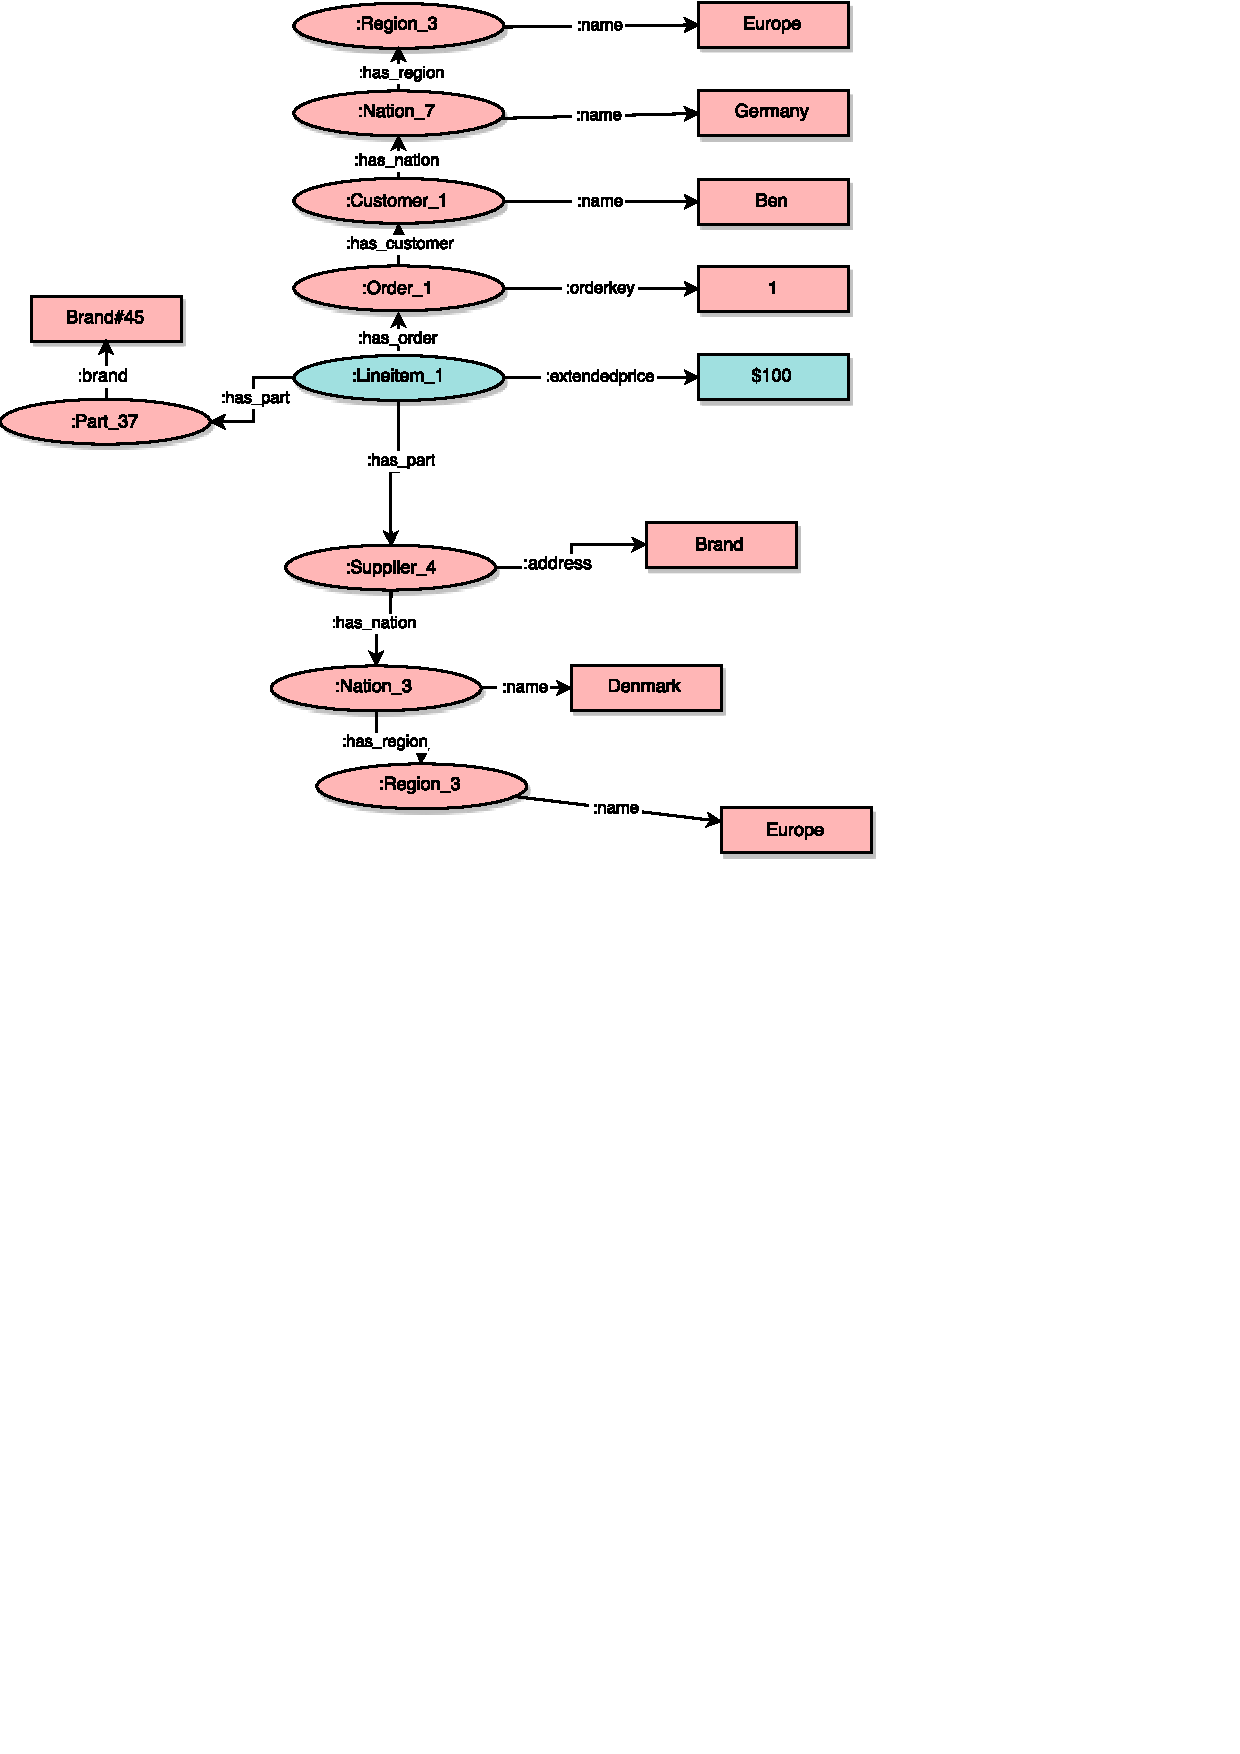
\includegraphics[trim=0 200 0 0,clip,width=\textwidth]{images/dataset_instance_example.pdf}
\end{figure}
\end{frame}

\begin{frame}{Building a Cube}
\begin{columns}
\column{.5\textwidth}
\begin{block}{Requirements}
\begin{itemize}
    \item Observations
    \item Level members
    \item Relations between levels
    \item Level attributes
\end{itemize}
\end{block}
\column{.5\textwidth}
    \begin{figure}
        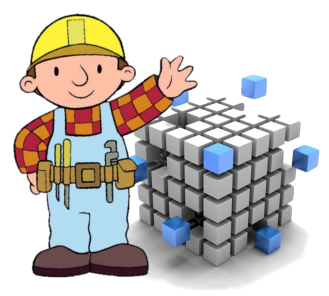
\includegraphics[width=0.8\textwidth]{images/cubeBuilder.png}
    \end{figure}
\end{columns}

\begin{block}{Candidate Frameworks}
\begin{itemize}
    \item QB\cite{dataCube}
    \item QB4OLAP\cite{DBLP:conf/semweb/EtcheverryV12}
\end{itemize}
\end{block}
\end{frame}

\newcommand{\patsec}{Patterns}
\section{\patsec}
\begin{frame}{\patsec}
    \begin{columns}
        \column{.5\textwidth}
        Snowflake Pattern
        \begin{figure}
            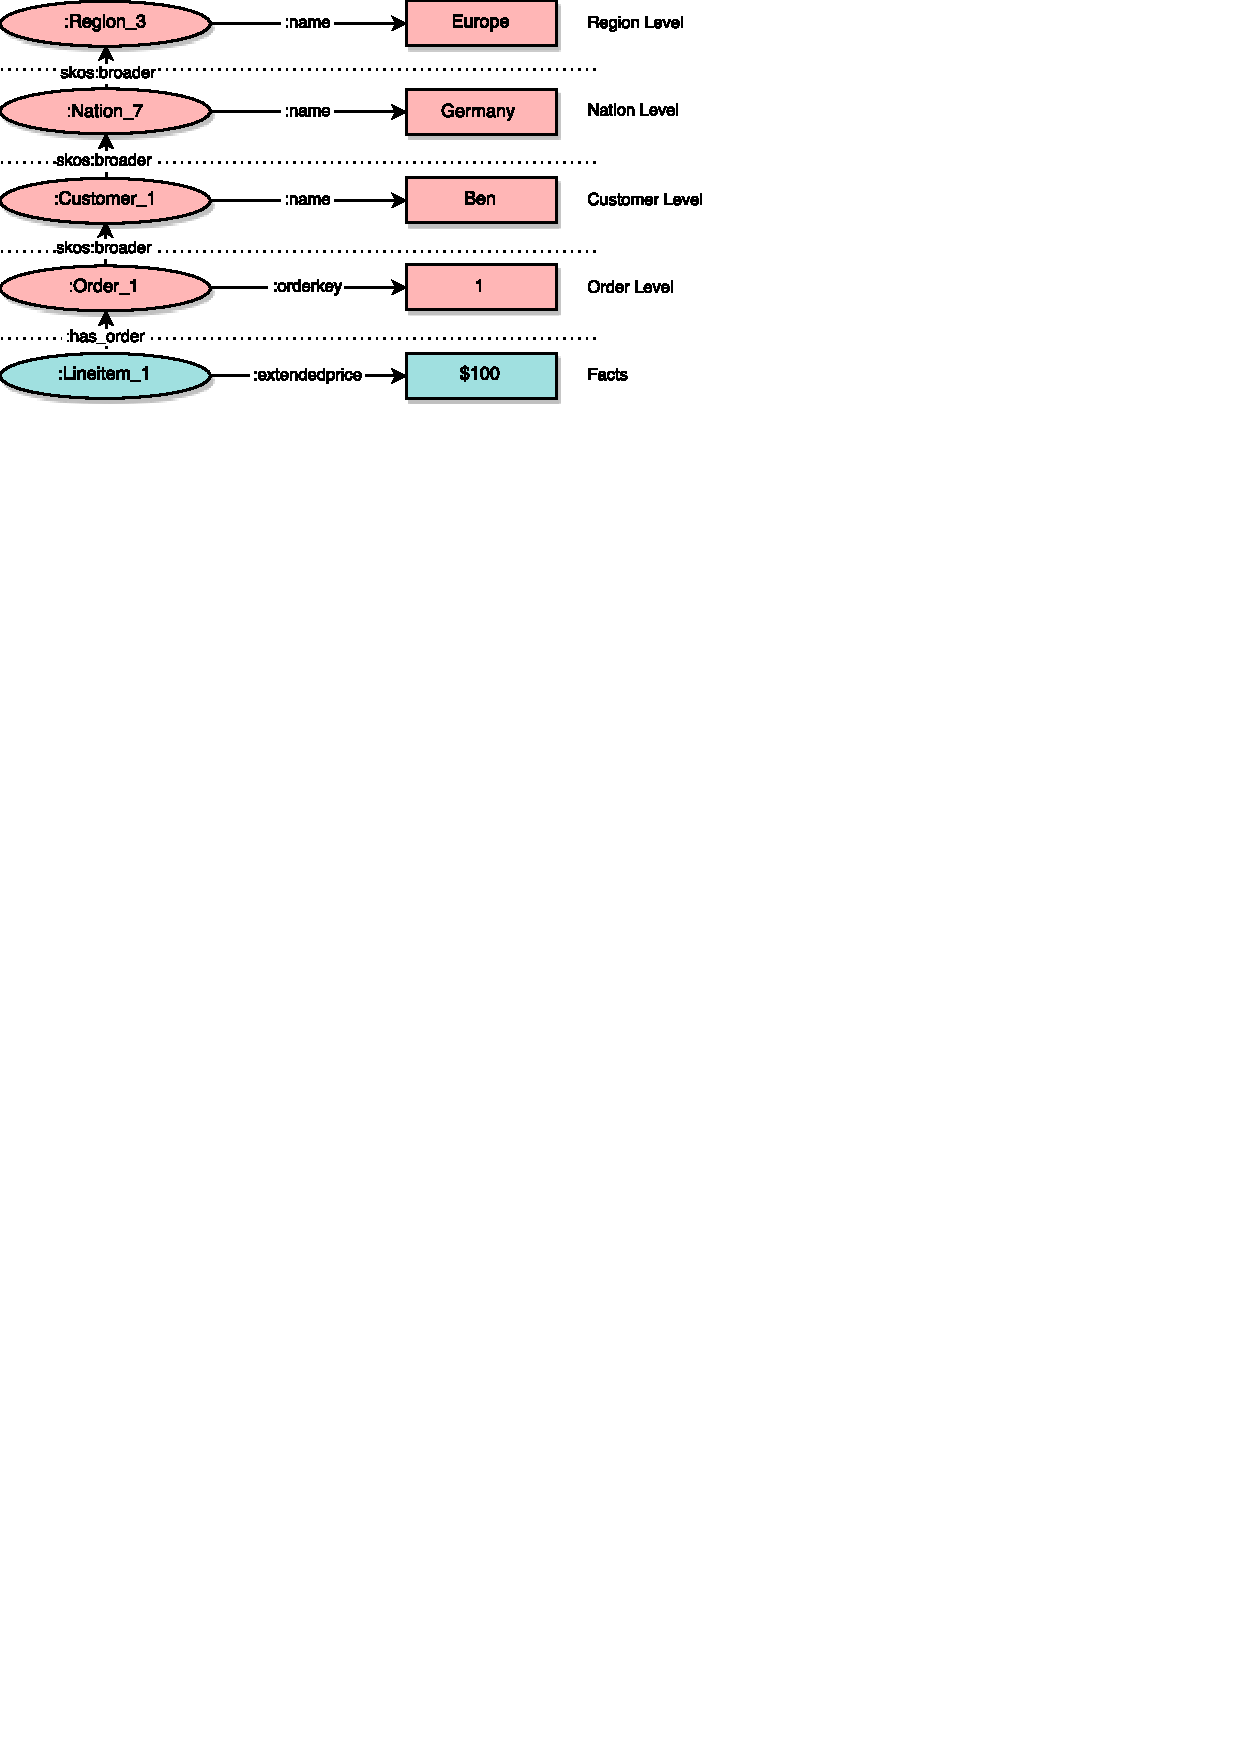
\includegraphics[trim=0 648 325 0,clip,width=0.5\textheight]{images/snowflakepattern.pdf}
        \end{figure}

        \column{.5\textwidth}
        Star Pattern
        \begin{figure}
            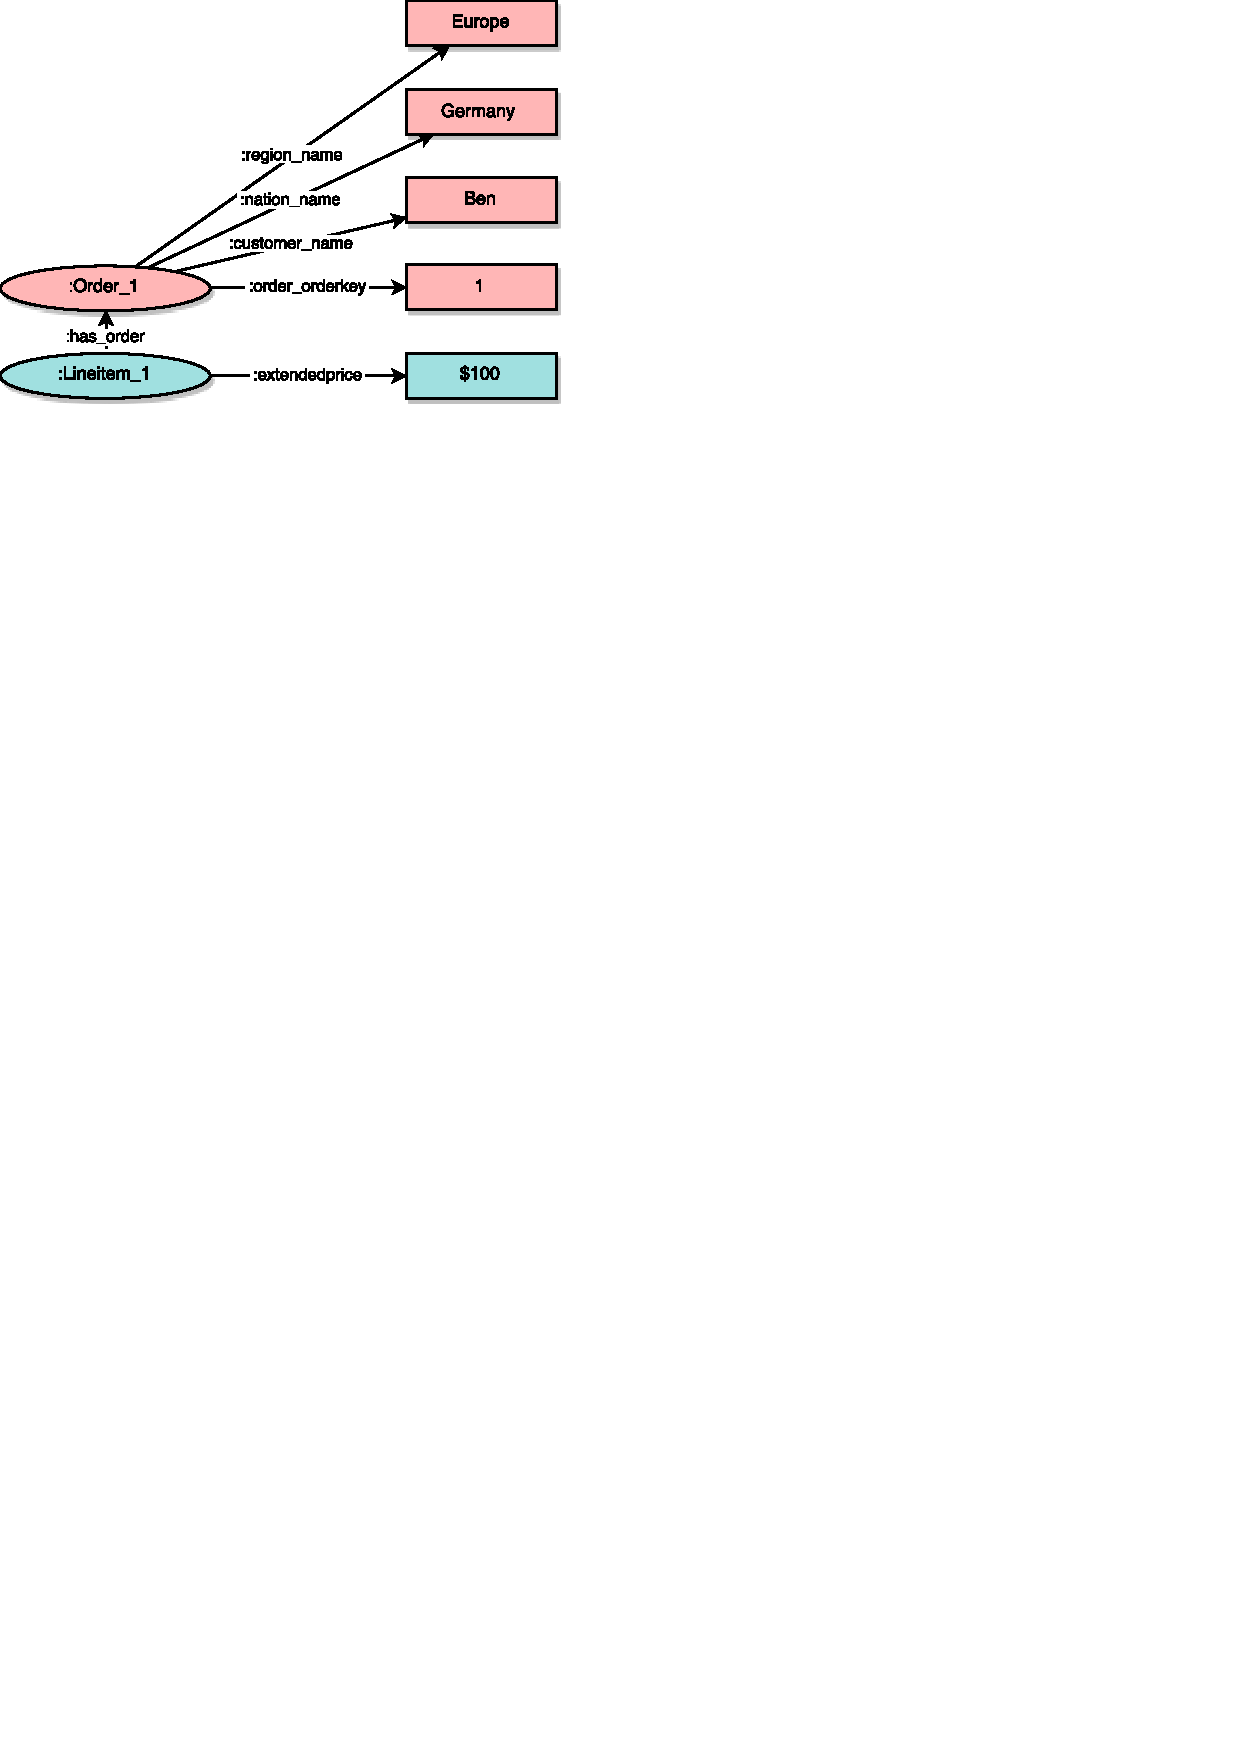
\includegraphics[trim=0 648 325 0,clip,width=.5\textheight]{images/starpattern.pdf}
        \end{figure}
        Fully Denormalized Pattern
        \begin{figure}
            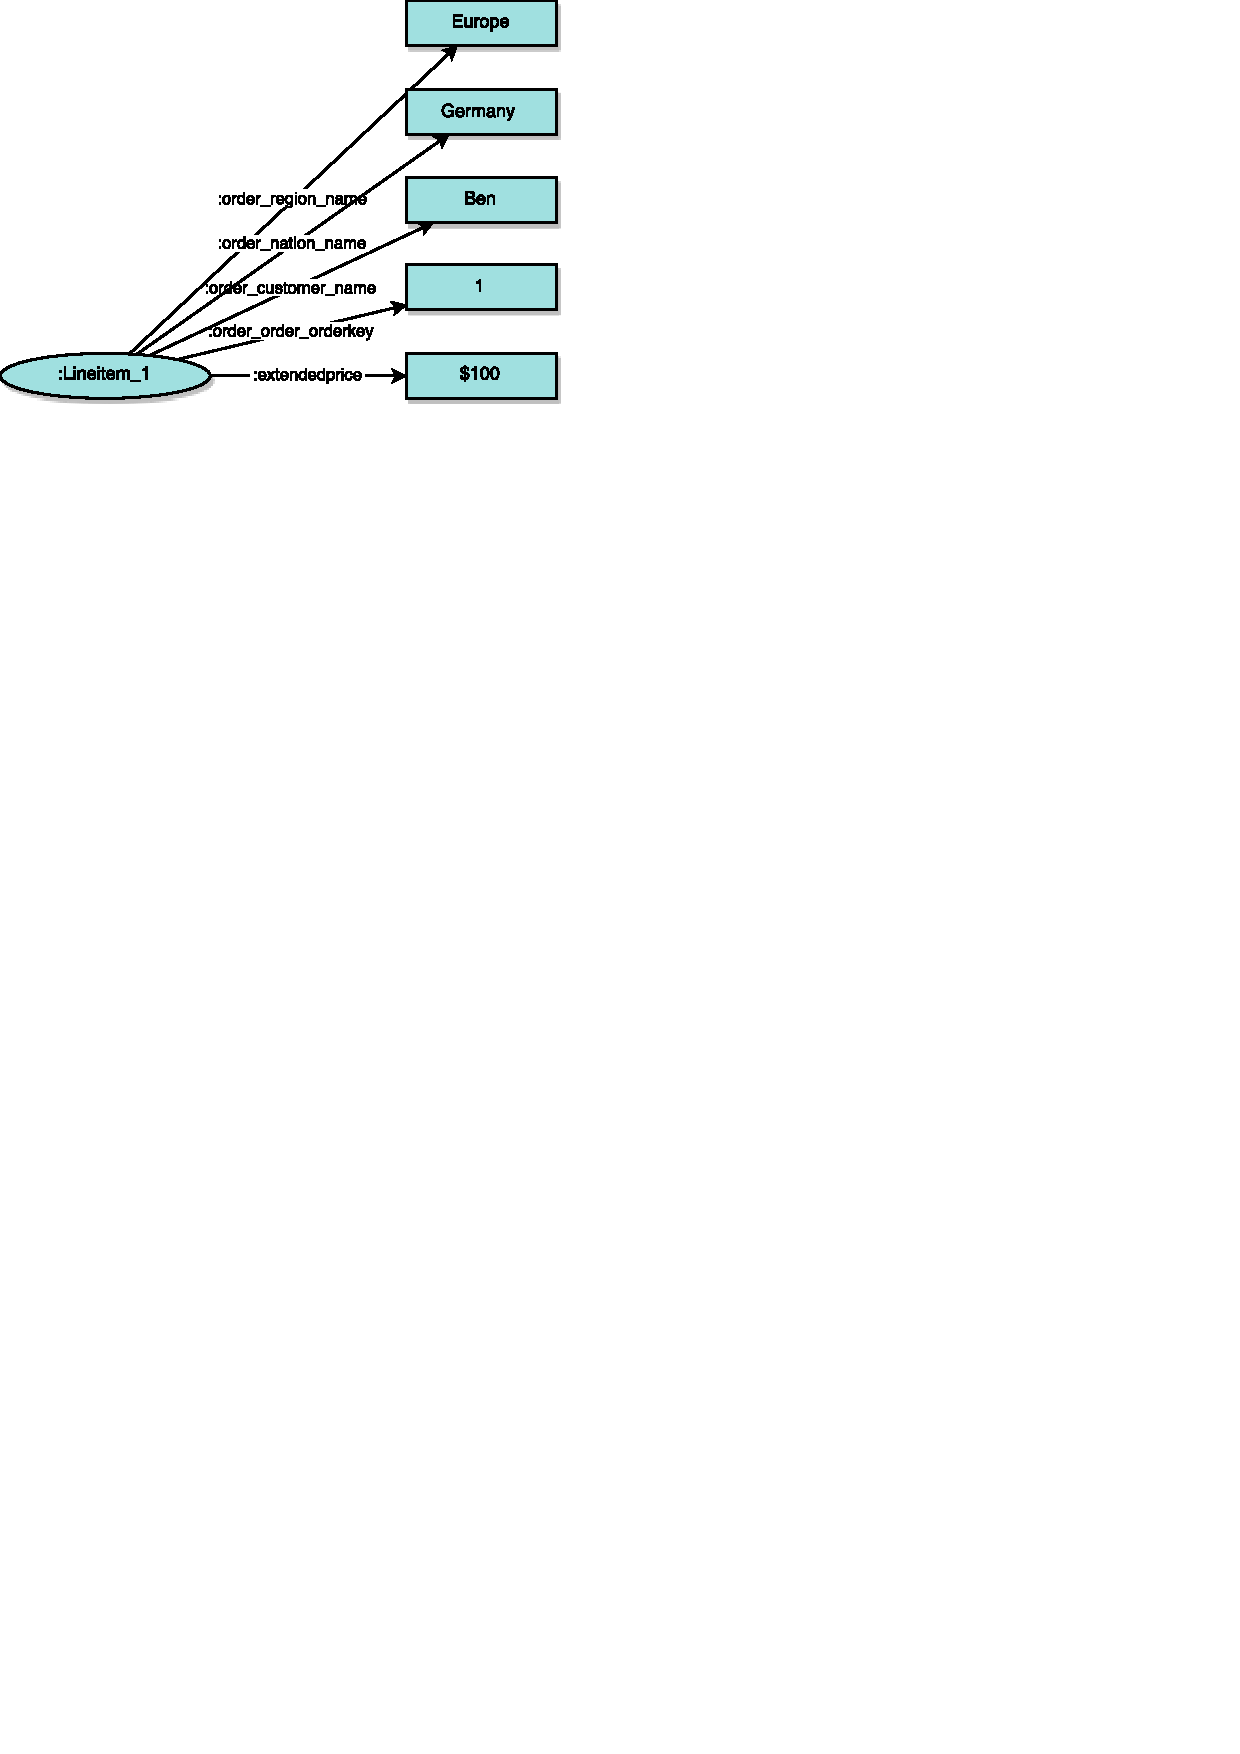
\includegraphics[trim=0 648 325 0,clip,width=.5\textheight]{images/denormalizedpattern.pdf}
        \end{figure}
    \end{columns}
\end{frame}

\begin{frame}{\patsec}
\framesubtitle{\snowpat}
    \begin{figure}
        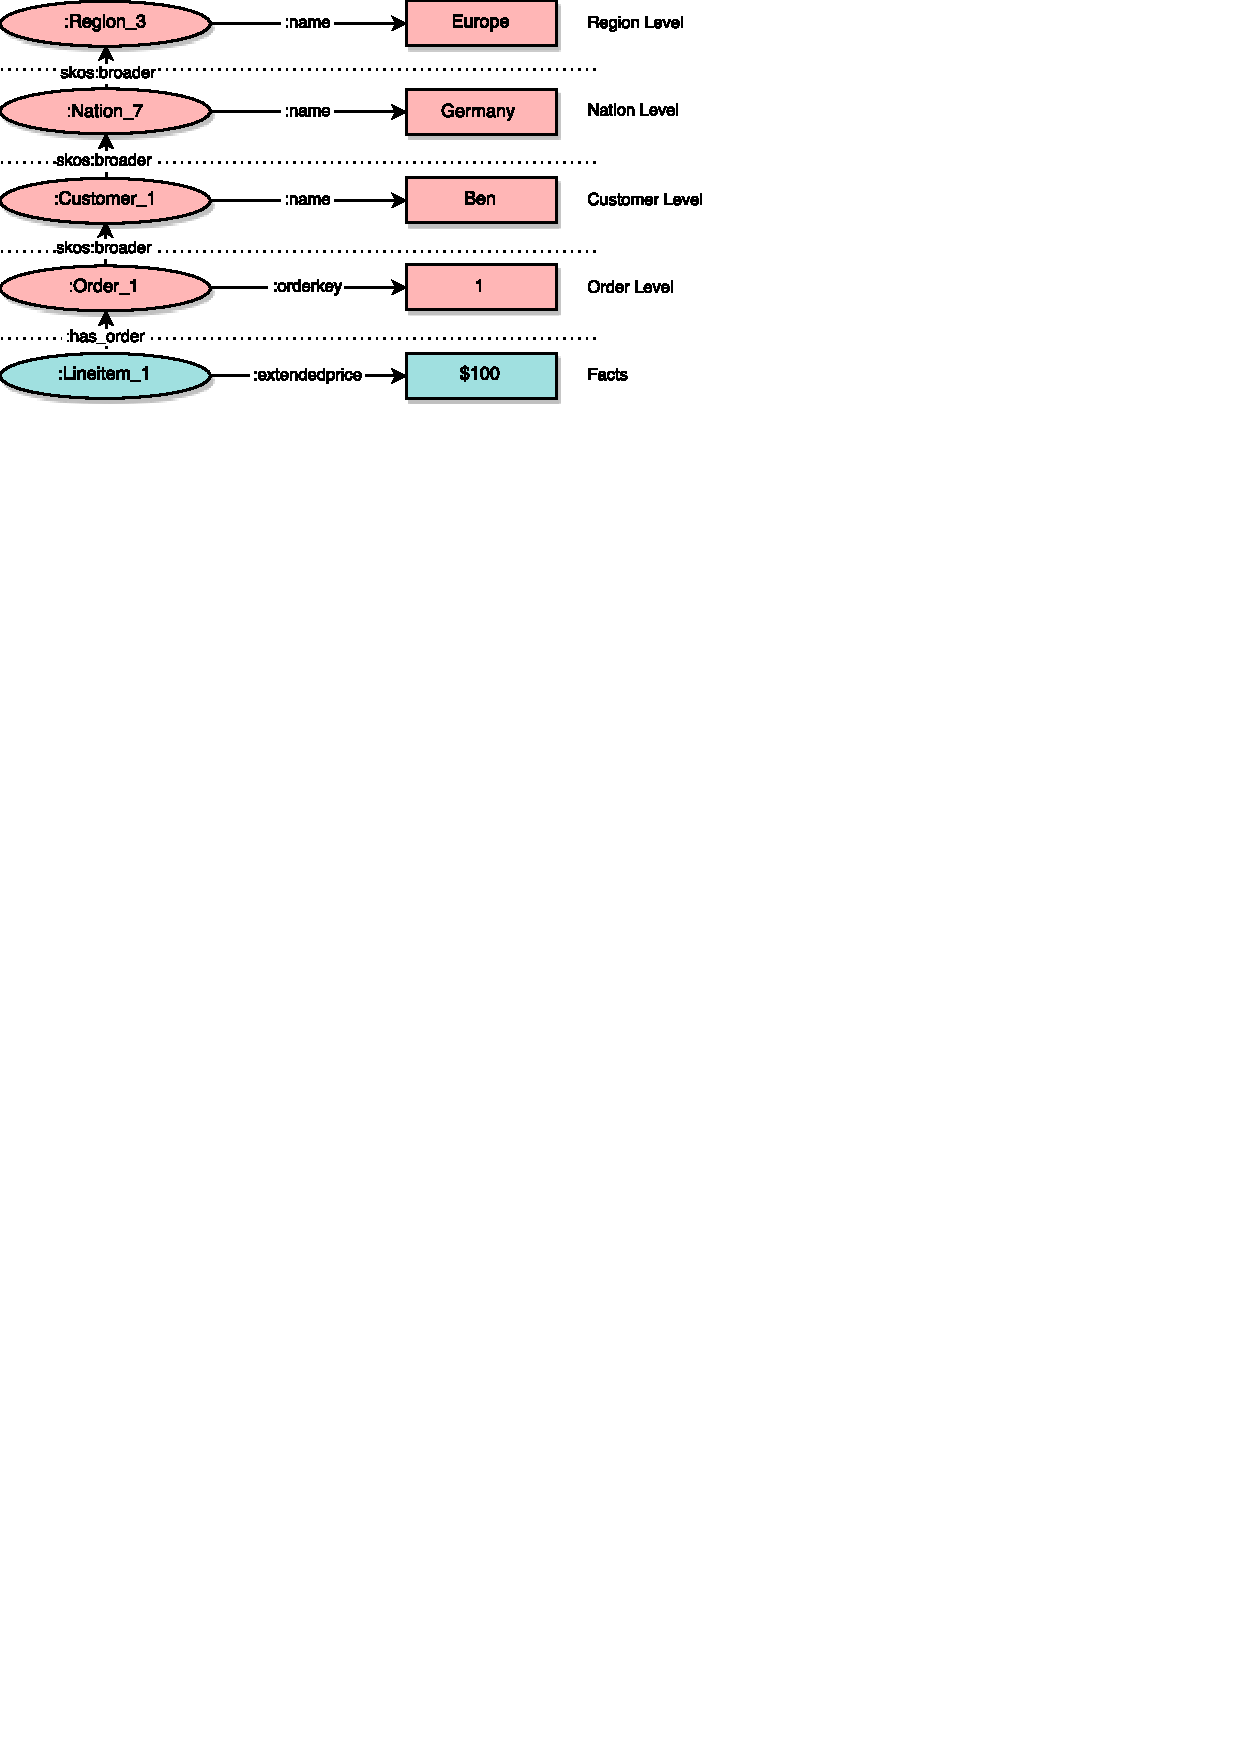
\includegraphics[trim=0 648 325 0,clip,width=1\textheight]{images/snowflakepattern.pdf}
    \end{figure}
\end{frame}

\begin{frame}{\patsec}
\framesubtitle{\starpat}
    \begin{figure}
        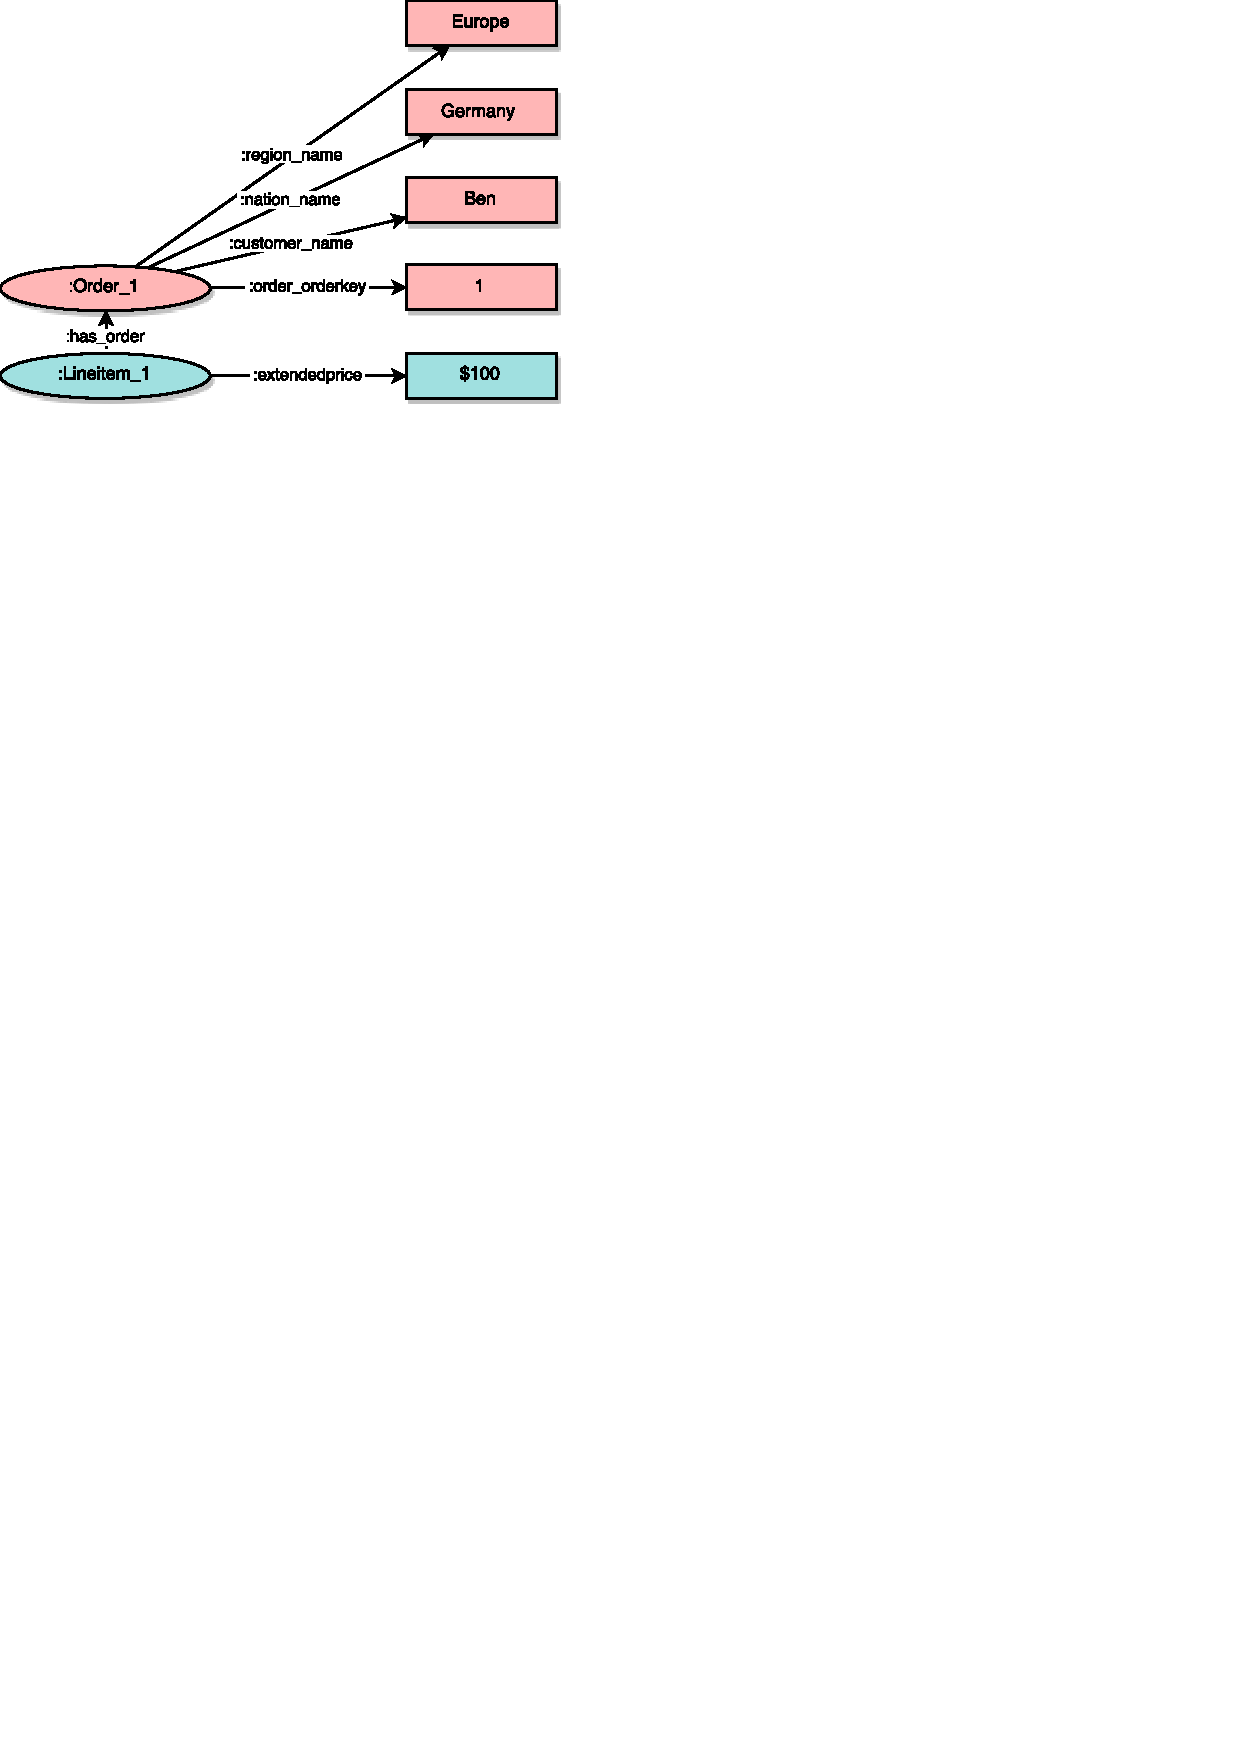
\includegraphics[trim=0 648 325 0,clip,width=1\textheight]{images/starpattern.pdf}
    \end{figure}
\end{frame}

\begin{frame}{\patsec}
\framesubtitle{\denormpat}
    \begin{figure}
        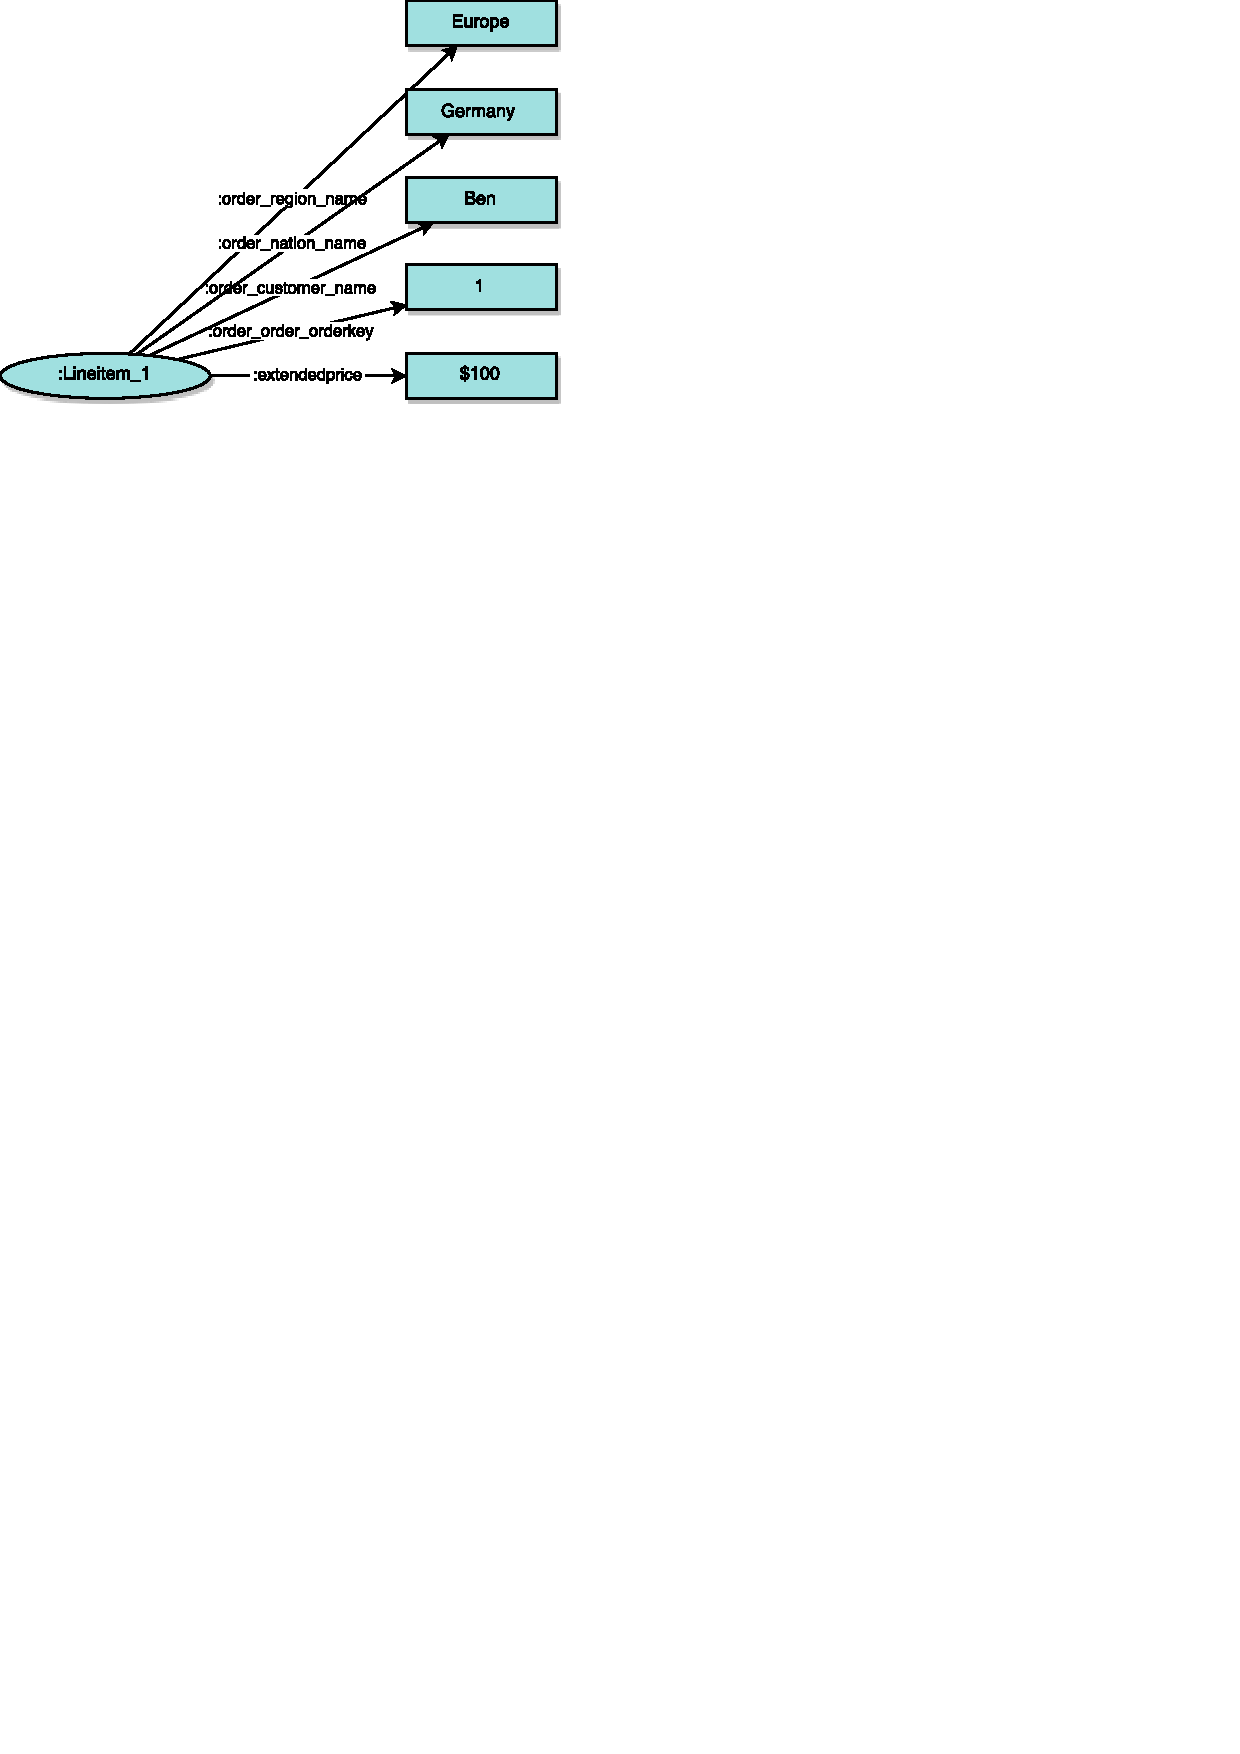
\includegraphics[trim=0 648 325 0,clip,width=1\textheight]{images/denormalizedpattern.pdf}
    \end{figure}
\end{frame}


\section{SWOD}

\begin{frame}{Semantic Web OLAP Denormalizations Algorithm}
\begin{columns}
    \column{0.5\textwidth}
    Input

    Output

    Features
    \column{0.5\textwidth}
    \begin{figure}
        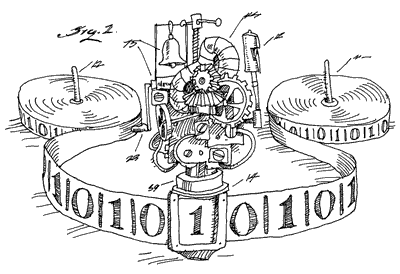
\includegraphics[width=\textwidth]{images/turingMachine.png}
    \end{figure}    
\end{columns}
\end{frame}


\begin{frame}{Problems}{Unballanced Heirichies}

\end{frame}

\begin{frame}{Problems}{Multiple Heirichies}

\end{frame}


\subsection{Unbalanced Hierarchies} 
\begin{frame}{\alg}
\framesubtitle{Unbalanced Hierarchies}
\begin{itemize}
    \item Paths from top level to leafs of different lengths
    \item<3-> E.g. the customer level of the orders dimension
\end{itemize}
\begin{figure}[tb]
    \begin{center}
        \invisible<1>{\includegraphics[]{images/alg-unbal-abstract-1}}
    \end{center}
\end{figure}
\end{frame}

\begin{frame}{\alg}
\framesubtitle{Unbalanced Hierarchies}
\begin{itemize}
    \item Naive approach from lowest level instances fails
    \item<2-> Move upwards on ontology and merge downwards on instances
\end{itemize}
\begin{figure}[tb]
    \begin{center}
        \includegraphics<1>[width=\textwidth]{images/alg-unbal-naive}
        \includegraphics<2>[width=\textwidth]{images/alg-unbal-base}
        \includegraphics<3>[width=\textwidth]{images/alg-unbal-merge-1}
        \includegraphics<4>[width=\textwidth]{images/alg-unbal-merge-2}
        \includegraphics<5>[width=\textwidth]{images/alg-unbal-merge-3}
        \includegraphics<6>[width=\textwidth]{images/alg-unbal-merge-4}
    \end{center}
\end{figure}
\end{frame}

\begin{frame}{\alg}
\framesubtitle{Unbalanced Hierarchies}
\begin{itemize}
    \item Dimension instances part of a number of levels
    \item Query level instances, which are unbalanced
\end{itemize}
\begin{figure}[tb]
    \begin{center}
        \includegraphics<1>[]{images/alg-unbal-onto-base}
        \includegraphics<2>[]{images/alg-unbal-onto-1}
    \end{center}
\end{figure}
\end{frame}

\subsection{Multiple Hierarchies}
\begin{frame}{\alg}
\framesubtitle{Multiple Hierarchies}
\begin{itemize}
    \item More than one path from bottom to top level
    \item Merge level instances of all hierarchies
\end{itemize}
\begin{figure}[tb]
    \begin{center}
        \includegraphics<1>[]{images/tpch-ps-hier}
    \end{center}
\end{figure}
\end{frame}

\begin{frame}{\alg}
\framesubtitle{Multiple Hierarchies}
\begin{figure}[tb]
    \begin{center}
        \includegraphics<1>[]{images/alg-multihier-base}
        \includegraphics<2>[]{images/alg-multihier-merge-1}
        \includegraphics<3>[]{images/alg-multihier-merge-2}
        \includegraphics<4>[]{images/alg-multihier-merge-3}
        \includegraphics<5>[]{images/alg-multihier-merge-4}
        \includegraphics<6>[]{images/alg-multihier-merge-5}
        \includegraphics<7>[]{images/alg-multihier-merge-6}
    \end{center}
\end{figure}
\end{frame}


\newcommand{\eval}{Evaluation}
\section{\eval}
\begin{frame}{\eval}
\framesubtitle{Load Time}
\begin{figure}
\footnotesize
\begin{tikzpicture}
\begin{axis}[
        xmode=log,
        ymode=log,
        xlabel={Scaling Factor},
        legend style={at={(1.025,0.975)},anchor=north west},
        ylabel={Load Time (s)}
    ]
\draw(axis cs:1,573642) node [fill=blue!20,draw=blue,circle,scale=1]{};
\addplot table[x index=0,y index=3,col sep=comma] {loadtime-accum.csv};
\addlegendentry{\denormpat}
\addplot table[x index=0,y index=2,col sep=comma] {loadtime-accum.csv};
\addlegendentry{\starpat}
\addplot table[x index=0,y index=1,col sep=comma] {loadtime-accum.csv};
\addlegendentry{\snowpat}% y index+1 since humans count from 1
\end{axis}
\end{tikzpicture}
\end{figure}
\end{frame}

\begin{frame}{\eval}
\framesubtitle{Number of Triples}
\begin{figure}
\footnotesize
\begin{tikzpicture}
\begin{axis}[
        xmode=log,
        ymode=log,
        xlabel={Scaling Factor},
        legend style={at={(1.025,0.975)},anchor=north west},
        ylabel={Number of Triples}
    ]
\draw(axis cs:1,414796747) node [fill=blue!20,draw=blue,circle,scale=1]{};
\addplot table[x index=0,y index=3,col sep=comma] {triples-lineitem.csv};
\addlegendentry{\denormpat}
\addplot table[x index=0,y index=2,col sep=comma] {triples-lineitem.csv};
\addlegendentry{\starpat}
\addplot table[x index=0,y index=1,col sep=comma] {triples-lineitem.csv};
\addlegendentry{\snowpat}% y index+1 since humans count from 1
\end{axis}
\end{tikzpicture}
\end{figure}
\end{frame}
\begin{frame}{\eval}
\framesubtitle{\QET}
\begin{figure}
\footnotesize
\begin{tikzpicture}
\begin{axis}[
        xmode=log,
        ymode=log,
        xlabel={Scaling Factor},
        legend style={at={(1.025,0.975)},anchor=north west},
        ylabel={Geo. Mean (s)}
    ]
\addplot table[x index=0,y index=3,col sep=comma] {results-avg.csv};
\addlegendentry{\denormpat}
\addplot table[x index=0,y index=2,col sep=comma] {results-avg.csv};
\addlegendentry{\starpat}
\addplot table[x index=0,y index=1,col sep=comma] {results-avg.csv};
\addlegendentry{\snowpat}% y index+1 since humans count from 1
\end{axis}
\end{tikzpicture}
\end{figure}
\end{frame}

%\begin{frame}{\eval}
%\framesubtitle{Timeouts}
%\begin{figure}
%\begin{tikzpicture}
%\begin{axis}[
%        xmode=log,
%        xlabel={Scaling Factor},
%        legend style={at={(0.025,0.975)},anchor=north west},
%        ylabel={Number of Timeouts}
%    ]
%\addplot table[x index=0,y index=3,col sep=comma] {timeouts.csv};
%\addlegendentry{\denormpat}
%\addplot table[x index=0,y index=2,col sep=comma] {timeouts.csv};
%\addlegendentry{\starpat}
%\addplot table[x index=0,y index=1,col sep=comma] {timeouts.csv};
%\addlegendentry{\snowpat}% y index+1 since humans count from 1
%\end{axis}
%\end{tikzpicture}
%\end{figure}


\begin{frame}{\eval}
\framesubtitle{Discussion}
\begin{itemize}
    \item Load times increase super-linearly with scaling factor
    \item Hard disk bottle neck when inserting triples
    \item \starpat 24--58\% slower than \snowpat
    \item \denormpat 41--1163\% slower than \snowpat
    \item Number of triples increase linearly
    \begin{itemize}
        \item Only small overhead for ontology
    \end{itemize}
\end{itemize}
\end{frame}

\definecolor{LRed}{rgb}{1,.8,.8}
\definecolor{MRed}{rgb}{1,.6,.6}
\definecolor{HRed}{rgb}{1,.2,.2}

\newcommand{\conc}{Summary and Future Work}
\section{\conc}
\begin{frame}{\conc}
\framesubtitle{Summary}
\begin{itemize}
    \item<+-> Logical patterns based on relational techniques
    \item<+-> SWOD algorithm converts between patterns
    \item<+-> TPC-H data converted to RDF, annotated with QB4OLAP
    \item<+-> Evaluation of patterns
    \begin{itemize}
        \item<1-3,+-> \denormpat not feasible
        \item<1-3,+-> \snowpat small, but slow \qet
        \item<1-3,+-> \starpat larger, but fast \qet\ -- good for many levels
    \end{itemize}
\end{itemize}
\end{frame}

\begin{frame}{\conc}
\framesubtitle{Future Work}
\begin{itemize}
    \item<+-> Query rewrites from \snowpat to other patterns
    \begin{itemize}
        \item Similar technique as for data conversion
        \item Consider variables
    \end{itemize}
    \item<+-> New version of QB4OLAP
    \begin{itemize}
        \item Hierarchies explicitly defined
    \end{itemize}
    \item<+-> Make SWOD module based
    \begin{itemize}
        \item Convert between all patterns
        \item Allow new patterns to be defined
    \end{itemize}
\end{itemize}
\end{frame}

%%%%%%%%%%%%%%%%%%%%%%%%%%%%%%%%%%%%%%%%%%%%%%%%%%%%%%%%%%%
%% Appendix
%%%%%%%%%%%%%%%%%%%%%%%%%%%%%%%%%%%%%%%%%%%%%%%%%%%%%%%%%%%
%\appendix
%\newcounter{finalframe}
%\setcounter{finalframe}{\value{framenumber}}
%
%
%
%\begin{frame}[c]{Extra}
%%\framesubtitle{}
%test
%\end{frame}
%
%\setcounter{framenumber}{\value{finalframe}}

\begin{frame}[allowframebreaks]
        \frametitle{References}
        \bibliographystyle{amsalpha}
        \bibliography{references.bib}
\end{frame}


\begin{frame}{\alg}
\framesubtitle{Example}
\begin{figure}[]
  \centering
  \includegraphics<+>[height=0.8\textheight]{images/00-SWOD.pdf}
  \includegraphics<+>[height=0.8\textheight]{images/0-SWOD.pdf}
  \includegraphics<+>[height=0.8\textheight]{images/1-SWOD.pdf}
  \includegraphics<+>[height=0.8\textheight]{images/2-SWOD.pdf}
  \includegraphics<+>[height=0.8\textheight]{images/3-SWOD.pdf}
  %\includegraphics<+>[height=0.8\textheight]{images/4-SWOD.pdf}
  \includegraphics<+>[height=0.8\textheight]{images/5-SWOD.pdf}
  \includegraphics<+>[height=0.8\textheight]{images/6-SWOD.pdf}
  \includegraphics<+>[height=0.8\textheight]{images/7-SWOD.pdf}
  \includegraphics<+>[height=0.8\textheight]{images/8-SWOD.pdf}
  \includegraphics<+>[height=0.8\textheight]{images/9-SWOD.pdf}
  \includegraphics<+>[height=0.8\textheight]{images/10-SWOD.pdf}
  \includegraphics<+>[height=0.8\textheight]{images/11-SWOD.pdf}
  \includegraphics<+>[height=0.8\textheight]{images/12-SWOD.pdf}
\end{figure}
\end{frame}

\begin{frame}{\alg}
\framesubtitle{Figure Licenses}
\begin{itemize}
    \item Workman -- Licence: CC BY 3.0 \\ Credit: www.clipartbest.com
    \item Cube -- Licence: CC BY 3.0 \\ Credit: www.clipartbest.com
    \item Turing machine \\ http://www.felienne.com/
\end{itemize}
\end{frame}

\end{document}